\documentclass[12pt,a4paper,oneside]{report}
\usepackage{indentfirst}
\usepackage{times}
\setlength\parindent{1cm}
\renewcommand{\baselinestretch}{1.50}\normalsize
\usepackage{anysize}
\marginsize{1.25in}{.75in}{1in}{1in}
\usepackage{graphics}
\usepackage{graphicx}
\usepackage{epsfig}
\usepackage[fleqn]{amsmath}
\usepackage{amsfonts}
\usepackage{textcomp}
\usepackage{graphicx}
\usepackage{setspace}
\usepackage{fancyhdr}
\usepackage{truncate}
\usepackage{nomencl} 
\usepackage{acronym}
\usepackage{array}
\usepackage{caption}\usepackage{subcaption}
\usepackage{subfig}
\usepackage[overload]{textcase}
\usepackage{listings}
\renewcommand{\nomname}{List of Abbreviations}
\usepackage{makeidx}
\makeindex
\makenomenclature
\newcommand{\quotes}[1]{``#1''}
\usepackage{titlesec}
\titleformat{\chapter}[display]
{\normalfont\Large\bfseries\centering}
{\chaptertitlename\ \thechapter}{15pt}{\LARGE}
\titleformat{\section}{\large\bfseries}{\thesection}{1em}{}
\titleformat{\subsection}{\normalsize\bfseries}{\thesubsection}{1em}{}
\renewcommand{\chaptermark}[1]{\markboth{ \emph{#1}}{}}

\printnomenclature[5em]
\pagestyle{fancy}
%\headheight 1pt
	\renewcommand{\footrulewidth}{1.2pt}
\renewcommand{\headrulewidth}{1.2pt}
\rhead{\scriptsize {\leftmark}}

\lhead{\small{College of Engineering, Cherthala \;\;\;\;\;\;\;\;\;\;\;\;\;\;\;\;\;\;}}
\rfoot{\thepage}
\cfoot{\empty}
\lfoot{\small{Department of Computer Science \& Engineering}}
\renewcommand{\figurename}{Fig.}
\begin{document}
\renewcommand\bibname{References}
\begin{titlepage}
\begin{center}
\LARGE{\textbf{Software Requirements Specification}}\\
\Large{\textbf{for}}\\

\begin{singlespace}
\LARGE{\textbf{Continues Integration Pipeline Implementation for Tech11Software}}\\
\end{singlespace}
\Large{{Prepared by  }}\\
\Large{\textit{\textbf{Aswin G SUGUNAN}     (\textbf{29})}}\\
\Large{\textit{\textbf{Jefin Jacob}    (\textbf{3})}}\\
\Large{\textit{\textbf{Nitin Suresh}   (\textbf{5})}}\\
\Large{\textit{\textbf{Vishnu Bose}   (\textbf{39})}}\\

\begin{singlespace}
\begin{flushleft}
%\small{\textbf{GROUP NUMBER: 2     \hspace{2.5in}      BATCH: S7 CSE B}}\\

\vspace{0.1in}
\small\textbf{{GUIDE :Mrs. Greeshma M G}}\\
\vspace{0.1in}
\small{\textbf{Remarks of  Guide :}}\\
\vspace{0.6in}
\small{\textbf{Remarks of Project Coordinators:}}\\

\end{flushleft}
\end{singlespace}


\vspace{0.1in}

\begin{figure}[h]
\begin{center}

\epsfig{width=1 in, file=logo.jpg}
\end{center}
\end{figure}
\begin{singlespace}
\small{\textbf{October 2015\\Department of Computer Science and Engineering\\College of Engineering, Pallippuram P O, Cherthala, Alappuzha-688541, \\Phone: 0478 2553416, Fax: 0478 2552714\\http://www.cectl.ac.in}}
\end{singlespace}
\end{center}
\end{titlepage}



\pagenumbering{roman}
\tableofcontents
\renewcommand*\thesection{\thechapter.\arabic{section}}
\newpage
\pagenumbering{arabic}
\setcounter{page}{1}
\pagestyle{fancy}
\headheight 26pt
\renewcommand{\footrulewidth}{1.2pt}
\renewcommand{\headrulewidth}{1.2pt}
\rhead{\scriptsize {\leftmark}}
%\chead{Middle top}
\lhead{\small{College of Engineering, Cherthala \;\;\;\;\;\;\;\;\;\;\;\;\;\;\;\;\;\;}}
\rfoot{\thepage}
\cfoot{\empty}
\lfoot{\small{Department of Computer Science \& Engineering}}
   

\chapter{INTRODUCTION}
\pagenumbering{arabic}
\setcounter{page}{1}
Software development, as we know it today, is a demanding area of business
with its fast-changing customer requirements, pressures of an ever shorter timeto-
market, and unpredictability of market. With the shift towards modern continuous deployment
pipelines, releasing new software versions early and often has become a concrete
option also for an ever growing number of practitioners. 
\par
Continuous delivery is a software development practice where
new features are made available to end users as soon as they have been
implemented and tested. In such a setting, a key technical piece of infrastructure
is the development pipeline that consists of various tools
and databases, where features 
ow from development to deployment and
then further to use.


\section{Purpose}
The objective of the project is to put in place a Continues Integration framework for product
development activities of Tech11 Software.This would enable the Tech11 team to rapidly bring a
product change or feature to production gaining market advantage.
This activities of this project will involve accessing different CI integration approaches and
solutions available,identify the feasibility of those solution by doing POCs and demos,fine tune the
final solution and set up the CI infrastructures,educate the developers on CI culture.

\newpage
\section{Document Conventions}
As this document is to be viewed by different class of people, to avoid ambiguity and to keep a standard, it has been documented in ieee format. This document have been organized into different sections and each section have been thoroughly analyzed and is presented here. 
\section{Intended Audience and Reading Suggestions}
\par
This SRS is intended for the usage by various level of people, such as from a novice, who is skilled with only basic understanding of a computer to high level programmers. This document is created for the use of various people like developers, project managers, testers, users, documentation writers etc. This document gives a detail on what our proposed system is what does it do, how it is implemented, for what it can be used, advantages over the existing systems. This document also specifies the functional and non functional requirements required by the user.
\par As we already said, this document is created with the intention of understanding this project by people from different levels of qualification and expertise and of different category. For users they need to understand only the services provided to them, so in the srs , they only need to go through introduction, product functions, user documentation, user interfaces and other non functional requirements. Designers need to go only through the interface requirements, product functions. Thus each category of people needs to proceed only through those section they require. This is achieved through well organizing of this document. 
\section{Product Scope }
The scope of the system is to help software developers to ensure new features are made available as soon as the program has been
implemented and tested. This product also helps in reducing the time needed to develop a software and also acts a guideline for future software developments




\chapter{OVERALL DESCRIPTION}
\section{Product Perspective}
\par
Continuous Integration is based on continuous performance of acts of integration of source code, testing, building and deployment in response to each change to the source code of the project submitted by the developer and for the use of tools for support of the development and testing by compliance with the established procedure automatically. The proposed system directs the user (developers) for time and cost effective production and solves majority of the Integration hell problem.

 \par Integration Hell refers to the point in production when members on a delivery team integrate their individual code. In traditional software development environments, this integration process is rarely smooth and seamless, instead resulting in hours or perhaps days of fixing the code so that it can finally integrate. Continuous Integration (CI) aims to avoid this completely by enabling and encouraging team members to integrate frequently (e.g., hourly, or at least daily).

\section{Product Functions}
\par
The CI frame work continuously monitors each development phase, automates the process of building, testing and reporting. 
\begin{figure}
\begin{center}
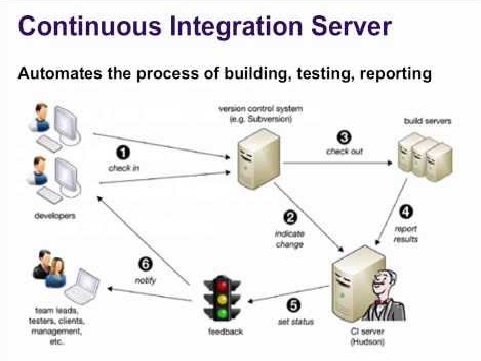
\epsfig{width=4 in, file=stages.jpg}
\end{center}
\end{figure} 
\par
The developer will push changes into the repository, example GitHub repository. The CI server some how notified these changes and pull the repository to check if there is any changes in the repository. Then the CI server clone the changes into the server and instruct the build server to check its correctness and build. The developers will be notified via email or other means.  


 \section{Operating Environment}
 The system is designed to work in various working implements.
 \section{Design and Implementation Constraints}
 Even though the system speeds up the development process, the end users needs to be familiarized with various tools recommended by the system.
\section{User Documentation}
 \begin{itemize}
 
 \item The system users will be provided with a user manual such that they can be familiarized with the product beforehand.
 \end{itemize}
 \section{Assumptions and Dependencies }
  
\par The Development environments should support repository plugging (recommended)and a sufficient speed Internet connection.
 


 \chapter{EXTERNAL INTERFACE REQUIREMENTS}
 \section{User Interfaces}
 \textbf{Main Screen:}\\
 It will have a login screen. The page will have each category listed clearly, with the selected candidate listed underneath its respective heading. At the very bottom of the page the user should see the "Go Back" and "Submit" buttons. 
 \begin{itemize}
 \item  Welcome screen 
 \item  Creating the Voters Database

\item  Modify the voters databases

\item  Delete the Voters database
\item  Creating the Election Instance
\item  The Voting on the Voters end



 \end{itemize}
 \section{Hardware Interfaces}

 The additional Infrastructure  used is Cloud Hosted Ubuntu system (IAAS). Herouku (PAAS)

\section{Software Interfaces}

\begin{itemize}

 
 \item Documentation : LaTeX
\item Version Control Framwork : Git,Svn
\item  Package Managment Framwork : Nexus
\item  Source Build Framwork : Jenkins
\item  Build Verification Framwork : PMD,CheckStyle,JUnit
\item Review Framework- : Gerrit
\item Verification and Review Tracking : BugZilla ,Trac
\item Deployment Framwork :Puppet,Chef 

\end{itemize}


\chapter{SYSTEM FEATURES}
\section{Frameworks}
\par



These are the high level system frameworks that has to be developed for the project
\begin{itemize}

\item  Version Control Framework
\item  Package Management Framework
\item  Source Build Framework
\item  Build Verification Framework
\item  Review Framework
\item  Verification and Review Tracking Framework
\item  Deployment Framework

\end{itemize}
\section{Functional Requirements}
The following are the functional requirements of E-Co-Operative\\
\textbf{REQ-1: Member Registration}\\
           \hspace{1.9 in} In order to use the system the voters must register to system. This explains the registration process. \\
           \newpage
           Normal flow of events: 
           \begin{enumerate}
           \item  Member enters the system homepage. 
           \item He clicks the "register now" button.
           \item The system prompts the application form. 
           \item He fills in the necessary information related with him in the application form. 
           \item He sends the request for registration by using "send" button. 
           \end{enumerate}
    \textbf{REQ-2: Approve Member }\\  
                    This describe how EA will approve the application form of voter and generate the new account to that voter Precondition.\\
                    Normal flow of events: 
                    \begin{enumerate}
                    \item EA selects the online voter application form from list. 
                    \item  EA checks the information of the applicant a
                  \item   If the the given information is correct 
                  \begin{enumerate}
                  \item EA approves the form by pressing "Approve" buton.
                  \item EA generates the new online account to this new voter 
                  \item EA prepares the username  and password send to member via message.
                  \end{enumerate}
                  \item if the given information is not correct  EA will inform voter about misinformation via message    
                    \end{enumerate}
\textbf{ REQ-3:Update Voters}\\                    
             This describe how EA updates online voters \\
    Normal flow of events: 
    \begin{enumerate}
    \item  The system checks online voters with respect to upcoming elections voters list.
    \item If the voter exists in the list, the system updates the voter with respect to official the voter information.
    \item If the voter does not exist in the list, the system deletes that voter from database.                  
    \end{enumerate}    
\textbf{REQ-4:Login/Logout} \\
This describes how the members log into the system \\
 Normal flow of events:
 \begin{enumerate}
 \item The user enters his login id and password
 \begin{enumerate}
 \item If the login and password is valid, a session is opened. 
 \item  The OTP password as  security. 
 \item The specific page of every user is loaded
  \item If the login or password is not valid, the login screen is redisplayed with an error message.
 \end{enumerate}
 \item The user click on the logout button.
 \begin{enumerate}
 \item The session is terminated.
 \item  The login screen is displayed.
\end{enumerate}   
\end{enumerate} 
\textbf{REQ-5: Voting }
    \begin{enumerate}
    \item Display Ballot Paper containing candidates names.
    \item Click favorable candidates to register vote.
    \end{enumerate}
\newpage
\textbf{REQ-6: View Election Results }\\
This describes the process of how the voters view the election results by using the system.\\
Normal flow of events: 
\begin{enumerate}
\item He clicks on the election results link.
\item He presses click on button "show results".
\item The system displays the required information according to the selected choices. 
\end{enumerate}
\par \textbf{REQ-7: Message Generation }\\
This describes the process of how the messages are send to the members.
\begin{enumerate}
\item If the membership is verified by admin, then send username and password to the corresponding members mobile number.
\item Send OTP password as  security to the corresponding members mobile number.
\end{enumerate} 


\chapter{OTHER NONFUNCTIONAL REQUIREMENTS} 
\section{ Performance Requirements}
\begin{itemize}


\item System should work smoothly with out lag.
\item Devement should not br interrupted. 
\item System shall support simultaneous users.
\item System shall give the user a user friendly interface.
\end{itemize}
\section{ Safety Requirements}
\begin{itemize} 
\item System use shall not cause any harm to human users. 
\end{itemize}   
\section {Security Requirements}
\begin{itemize}
\item	The Users must have individual as well as group passwords for accessing the system.
\item	Data handling have to be secured.
\end{itemize}
\newpage
\section {Software Quality Attributes	}
\begin{itemize}
\item	Maintainability.
\item The system have to continuously updated frequently.
\end{itemize}


%\chapter{Other Requirements}
%To implement this system, we require a storage area in server side which requires investment. This requires the need of a high speed network as to support simultaneous users. As everything is done online, it gives security and removes the chances for corruption from outside. The system can be accessed from mobile systems also, giving the users the facility to register their vote from anywhere they require.

\vspace{.4 in }

\newpage

\chapter{Glossary}

%\uppercase{\textbf{Appendix A: Glossary}}

%\addcontentsline{toc}{chapter}{\hspace{0.1in} Appendix A: Glossary}

\vspace{.1 in }
\begin{flushleft}
CI \hspace{1.6 in}:\hspace{.1 in} Continous Integration\\ 
\end{flushleft}

\begin{flushleft}
SRS\hspace{1.6 in}:\hspace{.1 in}Software Requirements Specification\\
\end{flushleft}

 

 \vspace{.1 in }
\hspace{.3 in} 


\end{document}
 
